% METODOLOGIA------------------------------------------------------------------

\chapter{METODOLOGIA}
\label{chap:metodologia}

Para uma melhor organização, a efetivação do trabalho é composta por duas partes, onde a primeira é a coleta de dados e, a segunda, o desenvolvimento da aplicação. 
Na segunda parte da execução do trabalho, será o desenvolvimento do algoritmo de reconstrução, que consistirá em quatro etapas, no qual, para cada etapa é desenvolvido uma rotina. 
Primeiro os dados serão preparados, em seguida serão refinados e filtrados, por fim, renderizados.
O produto final do processamento, será uma superfície tridimensional.
Cada parte está segmentada em etapas, no qual cada etapa é um processo a ser executado. Por conseguinte, a organização da metodologia apresenta os itens:

\begin{itemize}
    \addtolength{\itemindent}{2em}
    
    \item Coleta de dados
    \begin{itemize}
        \addtolength{\itemindent}{2em}
        
        \item Dados em simulação
        \item Dados \textit{in loco}
    \end{itemize}
    
    \item Desenvolvimento
    \begin{itemize}
        \addtolength{\itemindent}{2em}
        
        \item Pré-processamento
        \item Filtragem
        \item Reconstrução
        \item Comparação
    \end{itemize}
\end{itemize}
\hspace{1em}

A Figura \ref{fig:etapas} mostra as etapas do desenvolvimento da aplicação. Primeiramente, os dados são inseridos através de um \textit{dataset}, em verde são representados as etapas do pré-processamento, em amarelo são representados os processos de filtragem, o processo de reconstrução é representado em marrom, e por fim, a superfície é gerada.
A etapa de comparação requer duas superfícies na entrada do processo, para gerar a superfície resultante.


\begin{figure}[H]
    \centering
    \caption{Etapas do processo de desenvolvimento da aplicação.}
    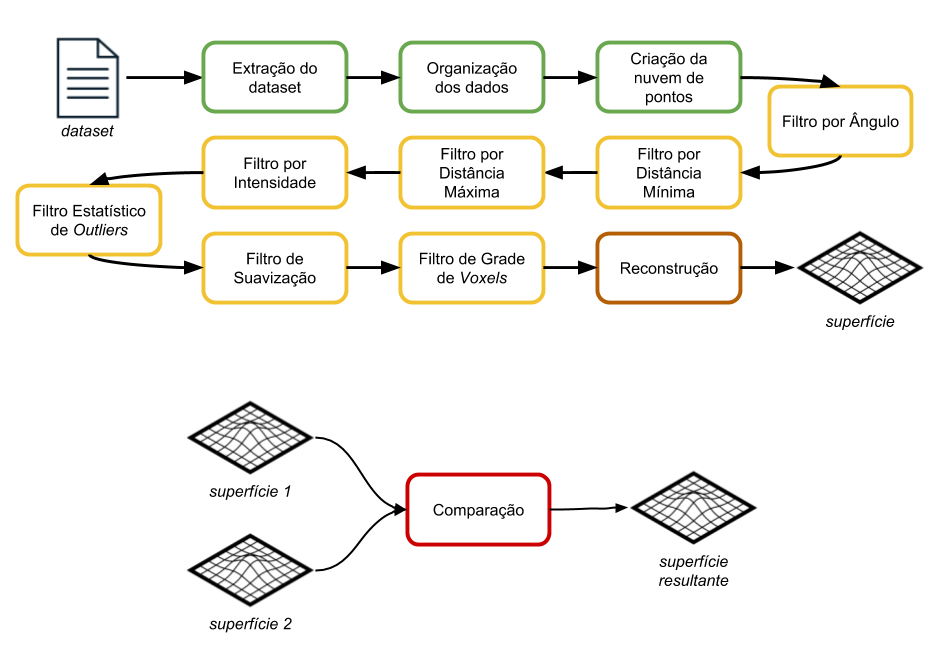
\includegraphics[scale=0.4]{dados/figuras/etapas.png}
    \label{fig:etapas}
\end{figure}

\section{Coleta de Dados}
\label{sec:coleta_dados}

A coleta de dados será realizada de duas formas: em simulação virtual do ambiente e \textit{in loco}. A coleta em simulação virtual facilita a obtenção de dados, por não ser necessário possuir um sensor ou robô e por dispensar planejamento logístico que uma saída de campo requer. Contudo, é importante fazer a coleta \textit{in loco}, pois, as informações obtidas em simulação não será próximo do real quanto às coletados em campo.

A obtenção de dados por simulação virtual contará com o auxílio de \textit{softwares} e ferramentas. O \textit{software} Gazebo  (seção \ref{sec:gazebo}) será o responsável por simular o ambiente virtual e executará dentro do ROS (seção \ref{sec:ros}) junto com outros pacotes, tais como o modelo de robô ROV (RexROV) e o simulador do sonar MSIS (seção \ref{sec:gpu_sonar_sim}). O RexROV é um modelo de robô desenvolvido pelos autores \cite{manhaes2016uuv} e está incluso no pacote \textit{UUV Simulator}.

A aquisição de dados pela coleta em campo, será realizado no local ainda a ser definido e será utlizado o ROV, modelo LBV300-5\footnote{Informações completas do modelo do ROV em: \url{http://www.teledynemarine.com/lbv300-5}} (Figura \ref{fig:rov_nautec}), do grupo do NAUTEC do C3. Acoplado ao robô, será utilizado o sensor MSIS modelo Tritech Micron Sonar\footnote{Informações completas do modelo do sensor em: \url{http://www.tritech.co.uk/media/products/small-rov-mechanical-sector-scanning-sonar-tritech-micron.pdf?id=e3070c7b}} que fará a captura dos dados.

\begin{figure}[H]
    \centering
    \caption{ROV utilizado no trabalho.}
    \label{fig:rov_nautec}
    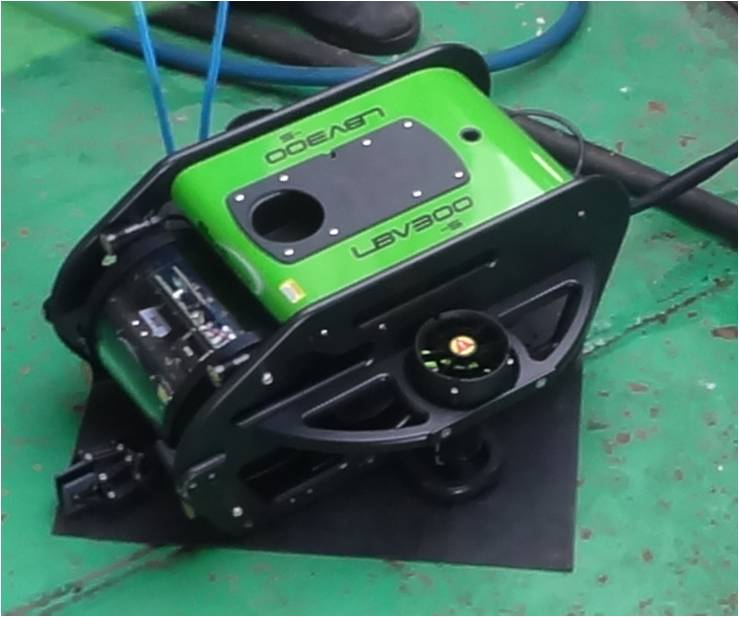
\includegraphics[scale=0.5]{dados/figuras/rov_furg.jpg}
\end{figure}

Para analisar a diferença entre os dados de ambas coletas, será realizada comparações entre os resultados obtidos em cada procedimento. Os materiais coletados, formarão um \textit{dataset} que servirá como entrada no algoritmo de reconstrução.

\section{Pré-processamento}

A etapa de pré-processamento serve para manipular os dados do \textit{dataset} e dispor em uma nuvem de pontos. Uma nuvem de pontos é um conjunto de pontos apresentados em um mesmo sistema de coordenadas tridimensional (Figura \ref{fig:point_cloud_example}) que possuem diversas finalidades, como criar modelos em 3D de animações, renderizações, objetos manufaturados, entre outros. 

\begin{figure}[H]
    \centering
    \caption{Nuvem de pontos gerada a partir de dados coletados por um sonar MSIS.}
    \label{fig:point_cloud_example}
    \begin{subfigure}[t]{0.32\textwidth}
        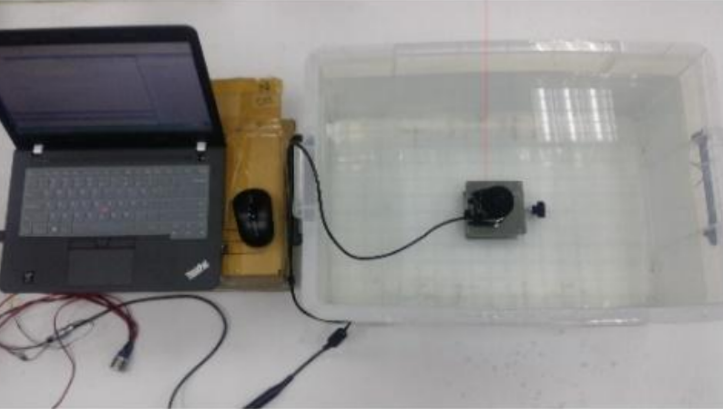
\includegraphics[width=\textwidth]{dados/figuras/point_cloud_example_tank.png}
        \caption{Sonar submerso no fundo do tanque d'água.}
    \end{subfigure}
    \hspace{3em}
    \begin{subfigure}[t]{0.32\textwidth}
        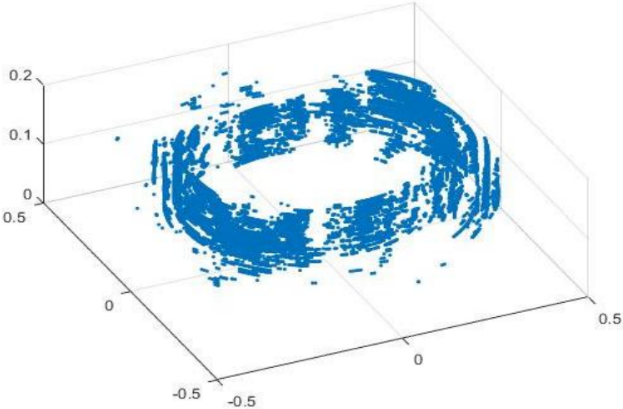
\includegraphics[width=\textwidth]{dados/figuras/point_cloud_example.png}
        \caption{Nuvem de pontos gerada.}
    \end{subfigure}
    \fonte{\cite{dong2017underwater}.}
\end{figure}

No final da fase de pré-processamento, o produto esperado é uma nuvem de pontos da superfície que foi escaneada pelo sonar. Esse resultado servirá como entrada para o próximo processo.

\section{Filtragem}
\label{sec:filtragem}

O processo de filtragem ou \textit{denoising} é composto por um conjunto de filtros em forma de funções que tem como objetivo remover informações desnecessárias da nuvem de pontos, como ruídos e \textit{outliers}\footnote{\textit{Outliers} é um termo da área da estatística utilizado para referênciar elementos atípicos ou observações que estão muito afastadas do restante da série.}.
O resultado da etapa de filtragem é uma nuvem de pontos mais limpa e legível, como ilustrado na Figura \ref{fig:point_cloud_denoise}. 
Desse modo, com um conjunto de pontos sem ruídos, torna mais simples o processo para ligar os pontos e formar um modelo tridimensional.

\begin{figure}[H]
    \centering
    \caption{Remoção de ruído em uma nuvem de pontos.}
    \label{fig:point_cloud_denoise}
    \begin{subfigure}[t]{0.45\textwidth}
        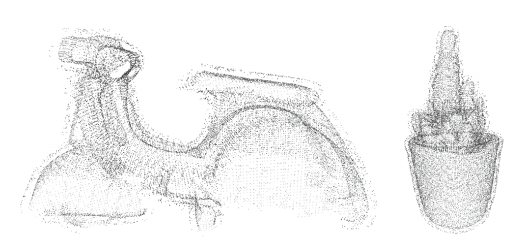
\includegraphics[width=\textwidth]{dados/figuras/noised.png}
        \caption{Nuvem de pontos com ruído.}
    \end{subfigure}
    \hspace{3em}
    \begin{subfigure}[t]{0.45\textwidth}
        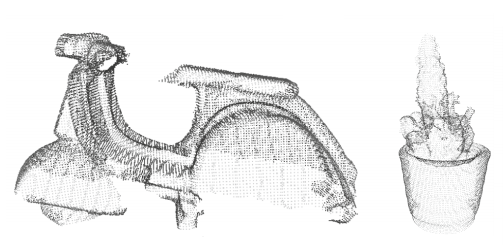
\includegraphics[width=\textwidth]{dados/figuras/denoised.png}
        \caption{Nuvem de pontos após remoção do ruído.}
    \end{subfigure}
    \fonte{Adaptado de \cite{arvanitis2017real}}
\end{figure}

Para realizar essa etapa, os filtros foram separados em dois grupos.
O primeiro grupo é composto por filtros simples, porém removem maior parte dos pontos desnecessários. 
O segundo conjunto é formado por filtros mais complexos onde muitos já estão implementados na PCL (Seção \ref{sec:pcl}).
Os filtros simples são representados pelo filtro por ângulo, filtro por intensidade e filtro por distância mínima, enquanto que os filtros complexos, são retratados pelo Filtro de Grade de \textit{Voxels}\footnote{Um \textit{voxel} é um \textit{pixel} que contém volume em um espaço tridimensional. Fazendo uma analogia, o \textit{voxel} seria um \textit{pixel} em 3D.}, Filtro de Suavização e o Filtro Estatístico de Remoção de \textit{Outliers}.

\subsection{Filtro por Ângulo}
\label{sec:angle_filter}

O filtro por ângulo, remove qualquer ponto que está fora da área cônica definida pelo ângulo horizontal $\theta$. Para esclarecer, na nuvem de pontos da Figura \ref{fig:angle_filter} são mostrados em cinza e em preto, os pontos descartados e mantidos pelo filtro, respectivamente.
O ângulo de abertura no sensor geralmente é configurável no próprio hardware, porém o critério do descarte fica por conta da aplicação, pois em um \textit{dataset}, os mesmos pontos que são inúteis em um trabalho podem ser úteis em outro. 
Por padrão, foi utilizado 120 graus para o ângulo $\theta$.

\subsection{Filtro por Distância Mínima}
\label{sec:distance_filter}

O filtro por distância mínima faz a remoção de pontos que estão próximos ao sensor, onde a presença de ruído costuma ser elevada. Da mesma forma como abordado no filtro anterior, os pontos em cinzas são descartados enquanto que os pretos são mantidos, como mostra a Figura \ref{fig:distance_filter}. Por padrão, o valor adotado para o raio de exclusão é de 5 metros, ou seja, serão descartados todos os pontos que estiverem até 5 metros de distância do sensor.

\subsection{Filtro por Intensidade}
\label{sec:intensity_filter}

Este processo remove os pontos que possuem baixo valor de intensidade. Os motivos para o sinal de intensidade ser baixo em um determinado ponto, pode ser:
    \begin{itemize}
        \item O ponto estar distante do sensor. Nesse caso, o sinal da onda estará fraco ao entrar em contato com o ponto, por conta da perda de energia para o meio ao longo da distância percorrida;
        \item O ângulo de incidência da onda com o ponto ser obtuso. Quando maior o ângulo de incidência entre a onda e o ponto, mais fraco será o sinal de retorno;
        \item A composição do objeto detectado pela onda. Quanto mais denso for o objeto, maior será o sinal de retorno.
    \end{itemize}

\begin{figure}[H]
    \centering
    \caption{Filtros simples de remoção de \textit{outliers}.}
    \begin{subfigure}[t]{0.4\textwidth}
        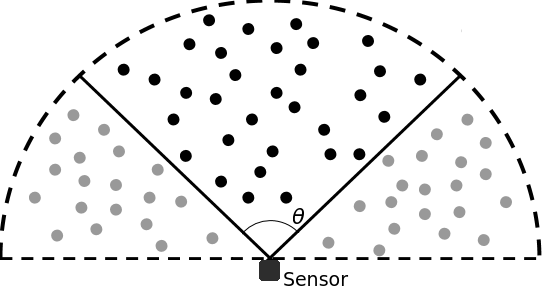
\includegraphics[width=\textwidth]{dados/figuras/angle_filter.png}
        \caption{Filtro por ângulo horizontal.}
        \label{fig:angle_filter}
    \end{subfigure}
    \hspace{3em}
    \begin{subfigure}[t]{0.4\textwidth}
        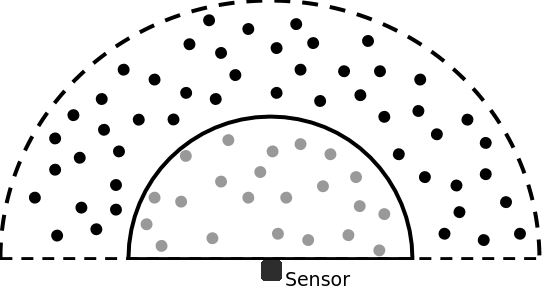
\includegraphics[width=\textwidth]{dados/figuras/distance_filter.png}
        \caption{Filtro por distância mínima.}
        \label{fig:distance_filter}
    \end{subfigure}
    \begin{subfigure}[t]{0.4\textwidth}
        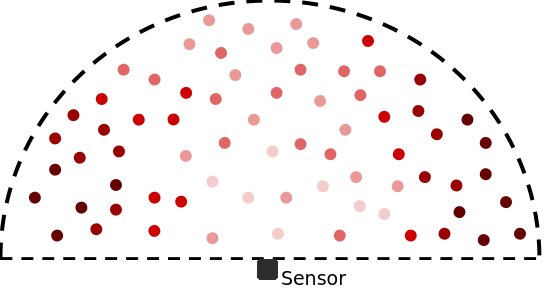
\includegraphics[width=\textwidth]{dados/figuras/intensity_filter.png}
        \caption{Filtro por intensidade.}
        \label{fig:intensity_filter}
    \end{subfigure}
\end{figure}

O exemplo ilustrado na Figura \ref{fig:intensity_filter}, mostra uma nuvem onde os pontos possuem diversos valores de intensidade. 
Quanto mais claro for o ponto, maior será o seu valor de intensidade do sinal de retorno. 
Portanto, o filtro descarta os pontos mais escuros na imagem.
Por padrão, é descartado todos os pontos que possuírem o valor de intensidade igual ou menor que 5\% da diferença entre o valor máximo e o valor mínimo de intensidade da nuvem de pontos.

\subsection{Filtro de Grade de \textit{Voxels}}
\label{sec:voxelgrid_filter}

O Filtro de Grade de \textit{Voxels} (do inglês \textit{Voxel Grid Filter}) tem a finalidade de diminuir a resolução/densidade e ordenar os pontos em uma nuvem. 
A Figura \ref{fig:voxelgrid_filter} exibe uma nuvem de pontos de entrada (esquerda) e o resultado gerado após aplicar o filtro (direita).

\begin{figure}[H]
    \centering
    \caption{Exemplo da aplicação do Filtro de Grade de \textit{Voxels}.}
    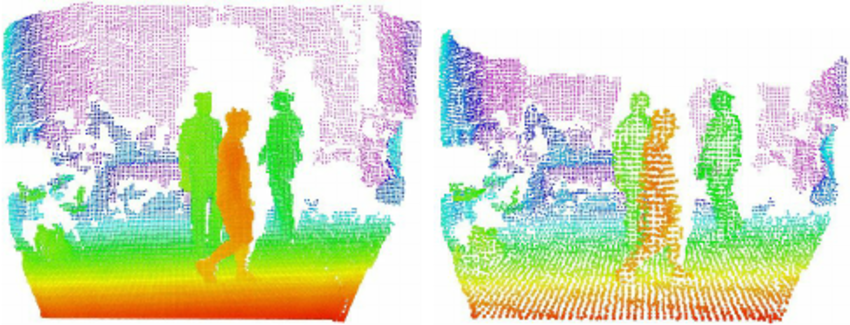
\includegraphics[scale=0.4]{dados/figuras/voxelgrid_filter.png}
    \label{fig:voxelgrid_filter}
    \fonte{\cite{munaro2012tracking}.}
\end{figure}

Para diminuir a quantidade de pontos e ordená-los, o algoritmo cria uma grade no conjunto de dados, onde os pontos são deslocados para o centroide da célula (\textit{voxel}) da grade em que estão contidos (o tamanho do \textit{voxel} é definido pelo usuário). A diminuição da quantidade e ordenação dos pontos facilita o processo de triangularização (etapa posterior responsável por transformar a nuvem de pontos em uma superfície).

\subsection{Filtro Estatístico de Remoção de \textit{Outliers}}
\label{sec:statistical_outlier_removal}

O SORF (Filtro Estatístico de Remoção de \textit{Outliers}, do inglês \textit{Statistical Outlier Removal Filter}) é um filtro da biblioteca PCL que é responsável por remover conjuntos de pontos que possuem uma densidade menor do que o restante dos conjuntos de pontos dentro da nuvem. 
A Figura \ref{fig:outlier_filter} exemplifica a aplicação do filtro. Na imagem à esquerda mostra a nuvem original que contém regiões em destaque, onde a densidade de pontos é menor que no restante da nuvem, enquanto que na imagem à direita mostra a remoção desses conjuntos de pontos.

\begin{figure}[H]
    \centering
    \caption{Exemplo do uso do SORF.}
    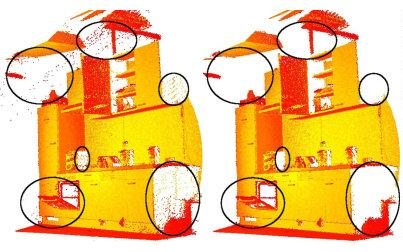
\includegraphics[scale=0.6]{dados/figuras/outlier_filter.jpg}
    \fonte{Adaptado de \cite{rusu2011pcl}.}
    \label{fig:outlier_filter}
\end{figure}

O filtro percorre a nuvem calculando, para cada ponto, a distância média entre seus pontos vizinhos (o número de vizinhos é definido pelo usuário). Assumindo o resultado como uma distribuição Gaussiana com uma média e um desvio padrão, todos os pontos cuja distância média estão fora de um intervalo definido pela média das distâncias globais e desvio padrão podem ser considerados \textit{outliers} e, portanto, removidos do conjunto de dados.

\subsection{Filtro de Suavização}
\label{sec:smoothing_filter}

O Filtro de Suavização é um filtro que está presenta na biblioteca PCL e é responsável por suavizar e reconstruir a superfície de pontos na nuvem. 
Para realizar o procedimento, o filtro utiliza o MLS (do inglês \textit{Moving Least Squares}), um método de reamostragem, desenvolvido por \cite{levin1998mls}, capaz de recriar partes ausentes ou suavizar superfícies por meio da interpolação polinomial entre pontos. 
Para exemplificar, a Figura \ref{fig:smoothing_filter} exibe uma superfície sem tratamento (imagem à esquerda) e a mesma superfície após a aplicação do filtro (imagem à direita).

\begin{figure}[H]
    \centering
    \caption{Exemplo do uso do Filtro de Suavização.}
    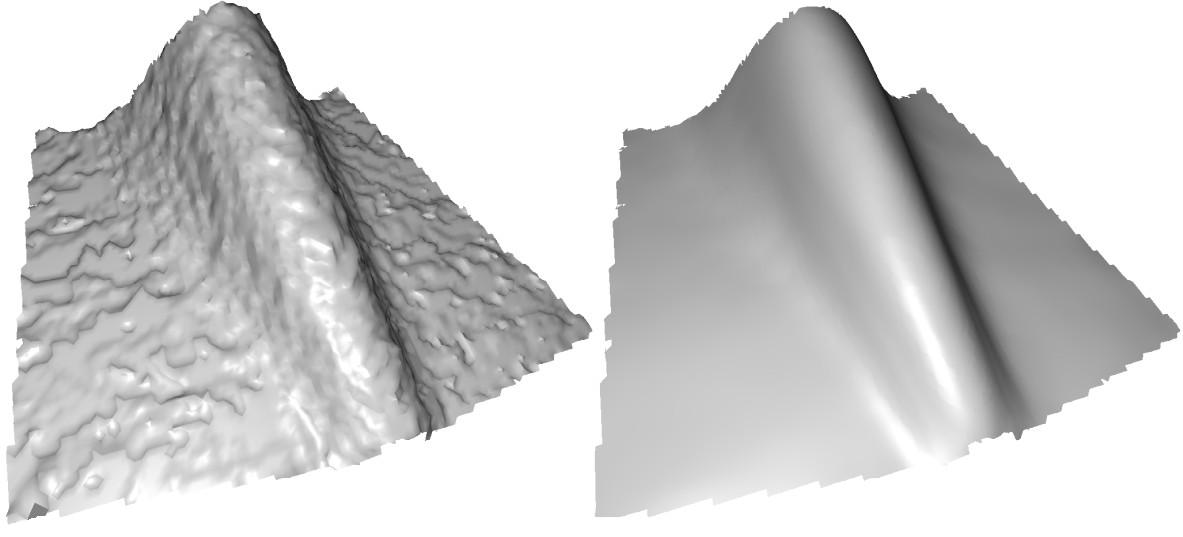
\includegraphics[scale=0.3]{dados/figuras/mls_filter.jpg}
    \fonte{Adaptado de \cite{ridel2015mls}.}
    \label{fig:smoothing_filter}
\end{figure}

No trabalho, o filtro é utilizado com o intuito de suavizar e corrigir boa parte do ruído e pequenos erros de medição de distância gerado nos dados, provenientes da movimentação do robô enquanto realiza a coleta.

\section{Reconstrução}
\label{sec:reconstrucao}

A reconstrução do modelo tridimensional é gerada a partir da nuvem de pontos, onde é obtido a forma final da superfície. 
Como exemplo, a Figura \ref{fig:reconstruction} mostra a reconstrução de um objeto passo a passo.

\begin{figure}[H]
    \centering
    \caption{Reconstrução de um objeto em 3D a partir de uma nuvem de pontos.}
    \label{fig:reconstruction}
    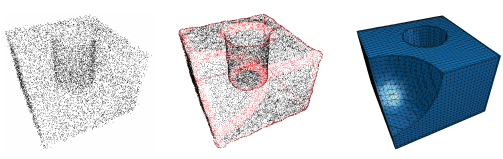
\includegraphics[scale=0.8]{dados/figuras/reconstruction.png}
    \fonte{Adaptado de \cite{jenke2006bayesian}.}
\end{figure}

Para dar forma à superfície é necessário uma lógica para ligar os pontos, para tal lógica chamamos de triangulação.
No trabalho, a triangulação é feita através da construção de triângulos sem fazer sobreposições, como ilustrado nos exemplos da Figura \ref{fig:triangulation}. 
Apesar do nome triangulação remeter à triângulos, ela pode ser constituída por qualquer espaço em simplexos ou polígono. 
Os simplexos são extensões de triângulos em outras dimensões, tais como segmentos de reta, tetraedros, e etc. 
Existem diversas formas para fazer a triangulação em um conjunto de pontos, entre elas estão a triangulação incremental e a triangulação do fecho convexo.

\begin{figure}[H]
    \centering
    \caption{Exemplos de modelos de triangulação.}
    \begin{subfigure}[t]{0.6\textwidth}
        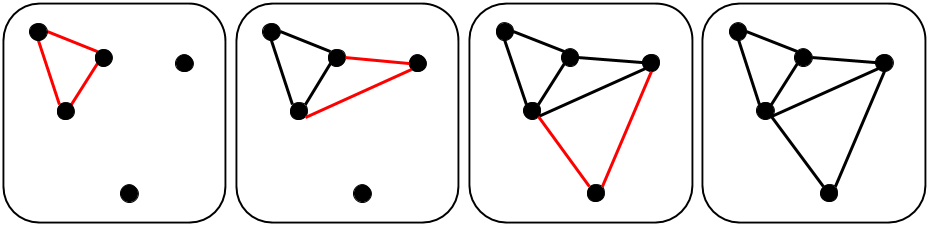
\includegraphics[width=\textwidth]{dados/figuras/triangulation_incremental.png}
        \caption{Triangulação Incremental}
        \label{fig:incremental_triangulation}
    \end{subfigure}
    \hspace{5em}
    \begin{subfigure}[t]{0.6\textwidth}
        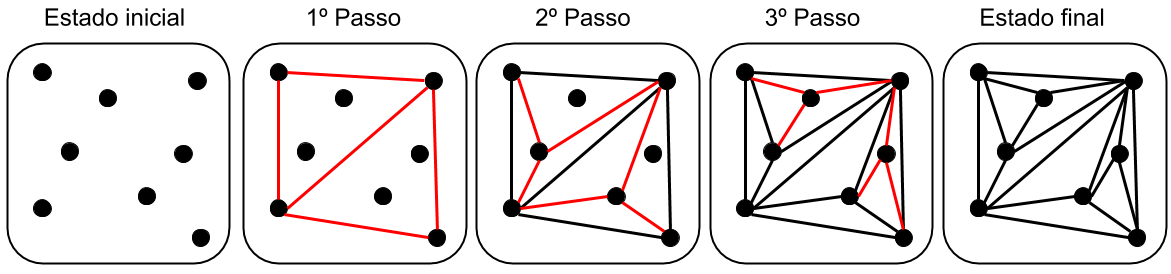
\includegraphics[width=\textwidth]{dados/figuras/triangulation_convex.png}
        \caption{Triangulação do Fecho Convexo}
        \label{fig:convex_triangulation}
    \end{subfigure}
    \label{fig:triangulation}
\end{figure}

Na Figura \ref{fig:incremental_triangulation} mostra a triangulação incremental, onde é realizada a construção de triângulos a partir da seleção aleatória do ponto inicial, seguindo a ligação pelo ponto mais próximo. 
Na Figura \ref{fig:convex_triangulation} mostra a triangulação do fecho convexo, na qual se realiza o fecho convexo do conjunto de pontos seguindo pela triangulação.
Após esse primeiro passo, para cada ponto no interior dos triângulos formados, se divide em mais três triângulos.

Fecho convexo (também conhecido como invólucro convexo ou envoltório convexo) são estruturas que englobam o conjunto de pontos, através da intersecção com seus pontos marginais. No plano, o fecho convexo é um polígono, enquanto que no espaço é representado por uma superfície (Figura \ref{fig:convex_hull}).

\begin{figure}[H]
    \centering
    \caption{Fecho convexo representado no plano (esquerda) e no espaço (direita).}
    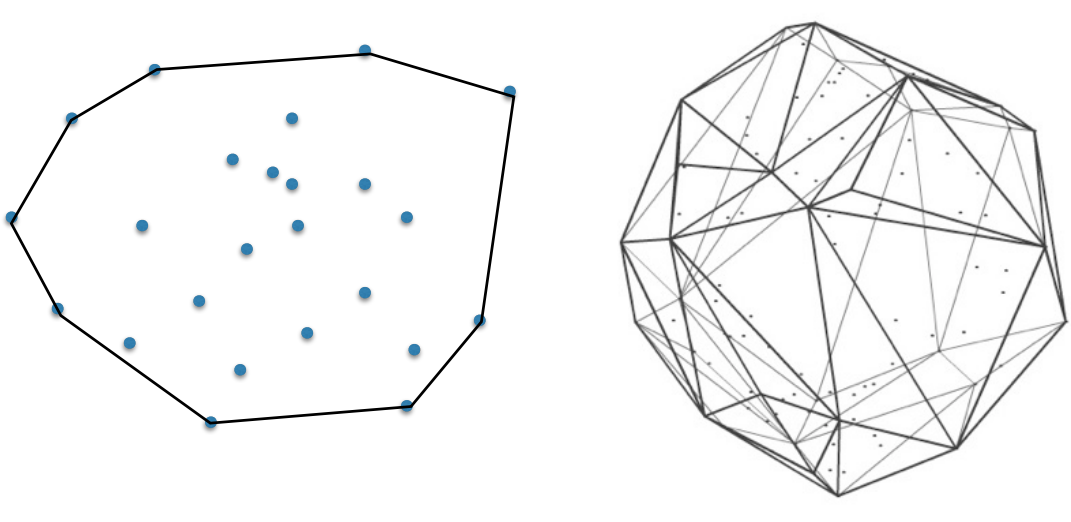
\includegraphics[scale=0.4]{dados/figuras/convex_hull.png}
    \label{fig:convex_hull}
\end{figure}

Uma triangulação nem sempre é adequada para um certo problema, pois os triângulos precisam ser parecidos com o triângulo equilátero (triângulos que não possuem ângulos internos agudos). Essas triangulações especiais usam critérios para definir triângulos, entre os modelos conhecidos existe a Triangulação de Delaunay.


\subsection{Triangulação de Delaunay}
\label{sec:delaunay}
A triangulação de Delaunay, proposto por \cite{delaunay1934sphere}, é o método responsável por fornecer uma triangulação com o maior ângulo mínimo, ou seja, os melhores triângulos de forma única, em um determinado conjunto de pontos. O método pode ser formulado e estudado no espaço euclidiano de dimensão $n$, mas para fins explicativos será definida e exemplificada apenas no plano.

\begin{figure}[H]
    \centering
    \caption{(a) Triangulação que não satisfaz o critério de Delaunay; (b) Triangulação de Delaunay.}
    \begin{subfigure}[t]{0.2\textwidth}
        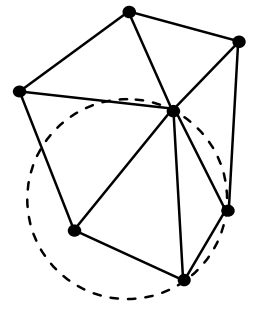
\includegraphics[width=\textwidth]{dados/figuras/delaunay1.png}
        \caption{}
        \label{fig:delaunay1}
    \end{subfigure}
    \hspace{3em}
    \begin{subfigure}[t]{0.3\textwidth}
        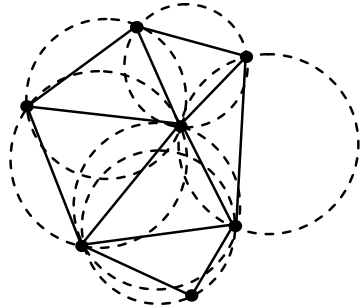
\includegraphics[width=\textwidth]{dados/figuras/delaunay2.png}
        \caption{}
        \label{fig:delaunay2}
    \end{subfigure}
    \fonte{Adaptado de \cite{piteri2007triangulacao}.}
    \label{fig:delaunay}
\end{figure}

Para a criação dos triângulos, se pode utilizar qualquer metodologia de triangulação (inclusive as que foram apresentadas na Figura \ref{fig:triangulation}). Após a criação, há uma verficação, que deve ser realizada em cada triângulo, definida pela regra do circuncírculo, que determina se o triângulo é ou não de Delaunay. 
A regra descreve que para cada triângulo da malha, é traçado um círculo que passa pelos três vértices do triângulo, se esse círculo conter apenas os 3 pontos do triângulo, então ele satisfaz a regra. 
Se haver mais de 3 pontos dentro, então é aplicada a troca (\textit{flip}) entre arestas contidas no círculo. 
Para explicar o termo \textit{flip}, observe a Figura \ref{fig:delaunay1}, onde o triângulo ABC não satisfaz a regra do circuncírculo, pois há outro vértice contído (D). 
Para resolver esse problema se utiliza o \textit{flip} entre os triângulos ABC e ACD, que faz a troca da aresta AC pela aresta DB. 
Refazendo a regra do circuncírculo nos triângulos, é possível observar (Figura \ref{fig:delaunay2}) que ambos são triângulos de Delaunay.

\begin{figure}[H]
    \centering
    \caption{Regra do circuncírculo que define se um triângulo é ou não de Delaynay.}
    \begin{subfigure}[t]{0.2\textwidth}
        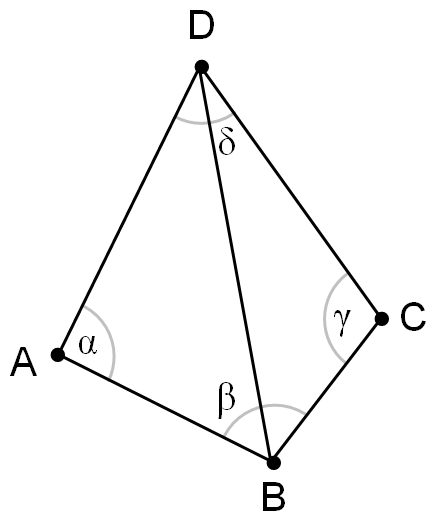
\includegraphics[width=\textwidth]{dados/figuras/delaunay_theorem1.png}
        \caption{}
        \label{fig:delaunay_theorem1}
    \end{subfigure}
    \hspace{2em}
    \begin{subfigure}[t]{0.27\textwidth}
        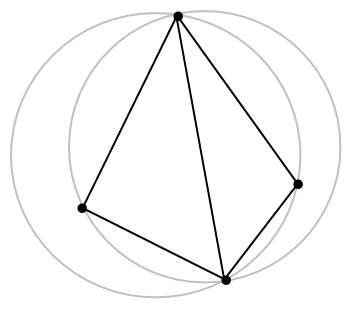
\includegraphics[width=\textwidth]{dados/figuras/delaunay_theorem2.png}
        \caption{}
        \label{fig:delaunay_theorem2}
    \end{subfigure}
    \hspace{2em}
    \begin{subfigure}[t]{0.2\textwidth}
        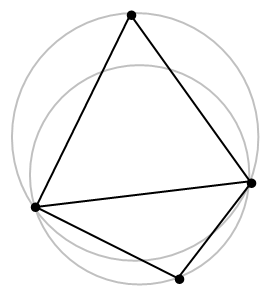
\includegraphics[width=\textwidth]{dados/figuras/delaunay_theorem3.png}
        \caption{}
        \label{fig:delaunay_theorem3}
    \end{subfigure}
    \label{fig:delaunay_theorem}
\end{figure}

Na Figura \ref{fig:delaunay_theorem} há outro exemplo de \textit{flip}. A Figura \ref{fig:delaunay_theorem2} mostra ambos triângulos que não obedecem a regra do circuncírculo. Realizando o \textit{flip} entre as arestas BD e AC, a regra se torna válida (Figura \ref{fig:delaunay_theorem3}). 
%Explicar como funciona a triangulação de Delaunay


\section{Comparação}
\label{sec:comparacao}

A comparação é a última etapa do processo de desenvolvimento. Essa parte é possível fazer a comparação entre dois modelos e determinar o quanto se perdeu ou ganhou em relação ao volume. Na fase de comparação será possível modelar coletas do mesmo local em diferentes períodos e fazer a comparação entre os resultados obtidos.



